\chapter{Terceiro Projeto: Sistema para Venda de Produtos}\label{cap:terceiroProjeto}
\epigraph{``\textit{A imaginação é mais importante que o conhecimento}''.}{Albert Einstein}

\lettrine[lines=4, lhang=0.1, lraise=0, loversize=0.2, findent=0.1em]{\textcolor{corAzulTema}{N}}{ESTE} Capítulo iremos construir mais um projeto completo, concluindo os conhecimentos básicos para que você possa construir praticamente qualquer tipo de sistema que lide com banco de dados, ou seja, aprenderemos a lidar com a implementação de cadastros que têm relacionamentos ``muitos para muitos''.


\section{Introdução}

Finalmente estamos aptos a construir uma aplicação Web em Java com a maioria das funcionalidades necessárias à maioria das aplicações Web que você desenvolverá na sua vida profissional. Iremos incrementar a aplicação criada no Capítulo~\ref{cap:primeiroProjeto} criando mais alguns cadastros e amarrando todos eles em um cadastro de vendas de produtos. Vamos lá!

Além de clientes, cidades e estados, criaremos mais três cadastros com inserção, alteração e remoção de registros: unidade de medida, produto e fornecedor. Com esses seis cadastros desenvolveremos a interface gráfica das vendas, onde poderemos gerar novas vendas e, após serem feitas, será permitido que sejam canceladas.

Na Figura~\ref{fig:cap08ModeloFisico} pode ser visto o modelo físico da base de dados \texttt{venda\_produtos}. Note que o nome da base é diferente do projeto anterior. Para esse projeto não disponibilizarei o script SQL para a criação da base de dados pois, além da estrutura, teremos algumas inserções já prontas para podermos testar. Para gerar a base, com o MariaDB/MySQL em execução, abra o modelo da base no MySQL Workbench, disponibilizado nos arquivos do projeto. Com o modelo aberto, clique no menu \destaque{\textit{Database}} e na opção \destaque{\textit{Forward Engineer...}} e siga o assistente. A base de dados, as tabelas, e os relacionamentos serão criados e várias inserções para as tabelas estado, cidade, cliente, fornecedor, unidade\_medida e produto.

\FloatBarrier
\begin{figure}[!htbp]
    \centering
    \caption{Diagrama do modelo físico da base de dados}
    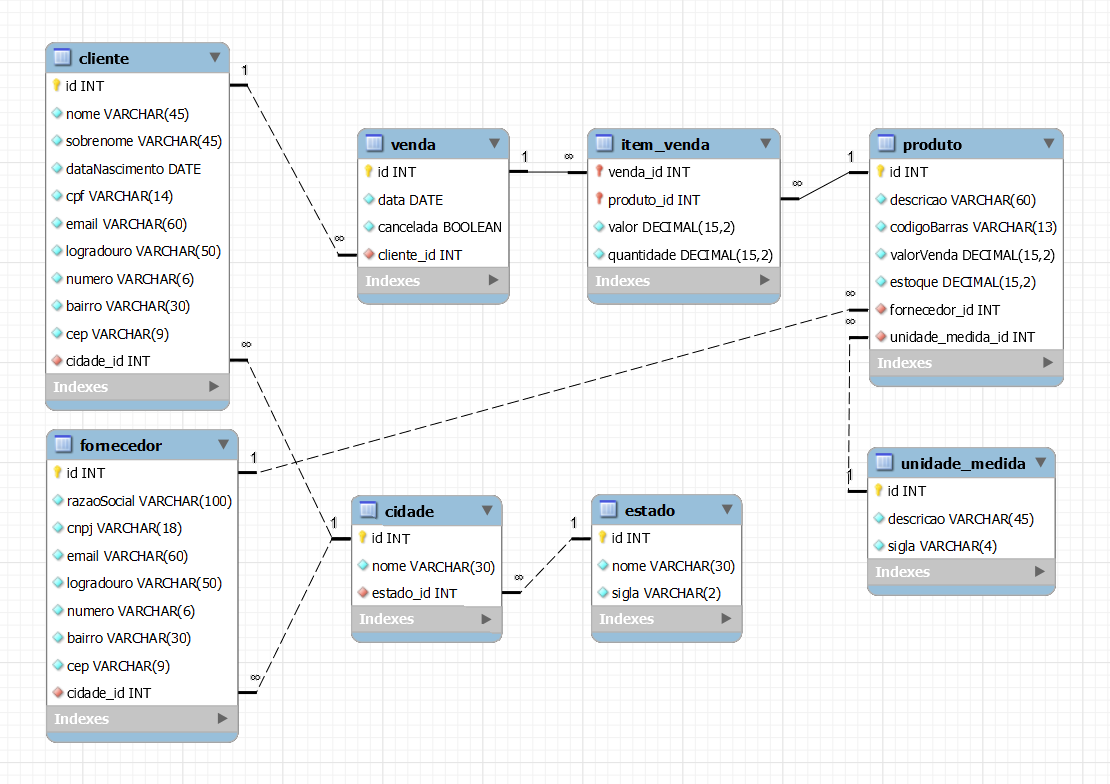
\includegraphics[scale=0.55]{imagens/cap08ModeloFisico}
    \\\textbf{Fonte:} Elaborada pelo autor
    \label{fig:cap08ModeloFisico}
\end{figure}
\FloatBarrier

O diagrama de classes do projeto pode ser visto Figura~\ref{fig:cap08DiagramaClasses}. Veja que a classe \texttt{ItemVenda} é a classe que fará o papel de viabilizar o relacionamento muitos-para-muitos entre produtos e vendas.

\FloatBarrier
\begin{figure}[!htbp]
    \centering
    \caption{Diagrama de classes das entidades}
    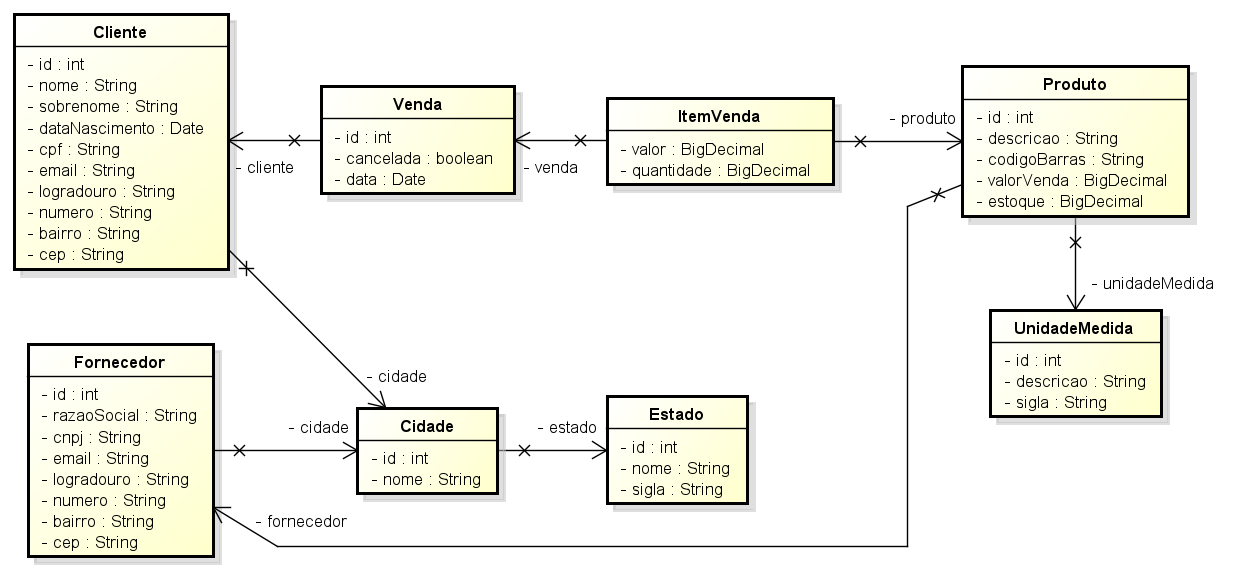
\includegraphics[scale=0.5]{imagens/cap08DiagramaClasses}
    \\\textbf{Fonte:} Elaborada pelo autor
    \label{fig:cap08DiagramaClasses}
\end{figure}
\FloatBarrier

Para que esse Capítulo não fique gigantesco, irei focar apenas nas novidades ou modificações que foram feitas em relação ao projeto anterior. Você poderá pegar o projeto pronto.


\section{Construindo o Sistema}

Esta seção será dividida em várias partes para que possamos organizar o que foi modificado em relação ao sistema anterior além, é claro, das funcionalidades novas. Os seis cadastros base são similares, então apenas um será detalhado o restante é por sua conta, basta ver o código pronto no projeto disponibilizado.


\subsection{Entidades e Validações}

Texto.

Listagem~\thechapter.\ref{listagem:projetos/capitulo08/VendaProdutos/src/java/vendaprodutos/entidades/Produto.java}.

\javaCode{Entidade ``Produto''\newline%
Arquivo: \texttt{vendaprodutos/entidades/Produto.java}}{projetos/capitulo08/VendaProdutos/src/java/vendaprodutos/entidades/Produto.java}

Usar exemplo do Produto.

Mostrar a entidade produto e falar dos validadores.

Mostrar o método de validação.

Texto.

Listagem~\thechapter.\ref{listagem:projetos/capitulo08/VendaProdutos/src/java/vendaprodutos/utils/Utils.java}.

\javaCode{Classe ``Utils'' com métodos estáticos utilitários\newline%
Arquivo: \texttt{vendaprodutos/utils/Utils.java}}{projetos/capitulo08/VendaProdutos/src/java/vendaprodutos/utils/Utils.java}


\subsection{DAO}

DAO genérico, AutoCloseable.

Listagem~\thechapter.\ref{listagem:projetos/capitulo08/VendaProdutos/src/java/vendaprodutos/dao/DAO.java}.

\javaCode{DAO genérico\newline%
Arquivo: \texttt{vendaprodutos/dao/DAO.java}}{projetos/capitulo08/VendaProdutos/src/java/vendaprodutos/dao/DAO.java}

Obtenção do identificador no salvar. ProdutoDAO.

Listagem~\thechapter.\ref{listagem:projetos/capitulo08/VendaProdutos/src/java/vendaprodutos/dao/ProdutoDAO.java}.

\javaCode{Código da classe ``ProdutoDAO''\newline%
Arquivo: \texttt{vendaprodutos/dao/ProdutoDAO.java}}{projetos/capitulo08/VendaProdutos/src/java/vendaprodutos/dao/ProdutoDAO.java}


\subsection{Servlets}

Falar do produto, pois tem BigDecimal. ProdutoServlet.

Listagem~\thechapter.\ref{listagem:projetos/capitulo08/VendaProdutos/src/java/vendaprodutos/controladores/ProdutosServlet.java}.

\javaCode{Código-fonte do Servlet ``ProdutosServlet''\newline%
Arquivo: \texttt{vendaprodutos/controladores/ProdutosServlet.java}}{projetos/capitulo08/VendaProdutos/src/java/vendaprodutos/controladores/ProdutosServlet.java}

\subsection{Tratamento de Erros}

Mostrar página de tratamento de erros.

Listagem~\thechapter.\ref{listagem:projetos/capitulo08/VendaProdutos/web/erro.jsp}.

\htmlCode{Página para exibição de erros\newline%
Arquivo: \texttt{/erro.jsp}}{projetos/capitulo08/VendaProdutos/web/erro.jsp}


\subsection{Cadastro de Vendas}

Falar das entidades e dos DAOs.

Venda

Listagem~\thechapter.\ref{listagem:projetos/capitulo08/VendaProdutos/src/java/vendaprodutos/entidades/Venda.java}.

\javaCode{Entidade ``Venda''\newline%
Arquivo: \texttt{vendaprodutos/entidades/Venda.java}}{projetos/capitulo08/VendaProdutos/src/java/vendaprodutos/entidades/Venda.java}

ItemVenda

Listagem~\thechapter.\ref{listagem:projetos/capitulo08/VendaProdutos/src/java/vendaprodutos/entidades/ItemVenda.java}.

\javaCode{Entidade ``ItemVenda''\newline%
Arquivo: \texttt{vendaprodutos/entidades/ItemVenda.java}}{projetos/capitulo08/VendaProdutos/src/java/vendaprodutos/entidades/ItemVenda.java}


VendaDAO

Listagem~\thechapter.\ref{listagem:projetos/capitulo08/VendaProdutos/src/java/vendaprodutos/dao/VendaDAO.java}.

\javaCode{Código da classe ``VendaDAO''\newline%
Arquivo: \texttt{vendaprodutos/dao/VendaDAO.java}}{projetos/capitulo08/VendaProdutos/src/java/vendaprodutos/dao/VendaDAO.java}

ItemVendaDAO

Listagem~\thechapter.\ref{listagem:projetos/capitulo08/VendaProdutos/src/java/vendaprodutos/dao/ItemVendaDAO.java}.

\javaCode{Código da classe ``ItemVendaDAO''\newline%
Arquivo: \texttt{vendaprodutos/dao/ItemVendaDAO.java}}{projetos/capitulo08/VendaProdutos/src/java/vendaprodutos/dao/ItemVendaDAO.java}

Falar do Servlet e da atualização do estoque. Falar do cancelamento da venda.

Listagem~\thechapter.\ref{listagem:projetos/capitulo08/VendaProdutos/src/java/vendaprodutos/controladores/VendasServlet.java}.

\javaCode{Código-fonte do Servlet ``VendasServlet''\newline%
Arquivo: \texttt{vendaprodutos/controladores/VendasServlet.java}}{projetos/capitulo08/VendaProdutos/src/java/vendaprodutos/controladores/VendasServlet.java}

Páginas

Listagem~\thechapter.\ref{listagem:projetos/capitulo08/VendaProdutos/web/formularios/vendas/listagem.jsp}.

\htmlCode{Código da listagem de Vendas\newline%
Arquivo: \texttt{/formularios/vendas/listagem.jsp}}{projetos/capitulo08/VendaProdutos/web/formularios/vendas/listagem.jsp}


Listagem~\thechapter.\ref{listagem:projetos/capitulo08/VendaProdutos/web/js/formularios/vendas/listagem.js}.

\javaScriptCode{\textit{Script} para cancelamento de Vendas\newline%
Arquivo: \texttt{/js/formularios/vendas/listagem.js}}{projetos/capitulo08/VendaProdutos/web/js/formularios/vendas/listagem.js}


Listagem~\thechapter.\ref{listagem:projetos/capitulo08/VendaProdutos/web/formularios/vendas/novo.jsp}.

\htmlCode{Formulário de cadastro de novas Vendas\newline%
Arquivo: \texttt{/formularios/vendas/novo.jsp}}{projetos/capitulo08/VendaProdutos/web/formularios/vendas/novo.jsp}


Listagem~\thechapter.\ref{listagem:projetos/capitulo08/VendaProdutos/web/js/formularios/vendas/novo.js}.

\javaScriptCode{\textit{Script} para tratamento de novas Vendas\newline%
Arquivo: \texttt{/js/formularios/vendas/novo.js}}{projetos/capitulo08/VendaProdutos/web/js/formularios/vendas/novo.js}


\section{Resumo}

Neste Capítulo construímos uma aplicação Web completa para a venda de produtos. Utilizamos para isso tudo que aprendemos até agora. Com isso você já é capaz de implementar a maioria dos tipos de cadastros que aparecerão em sistemas do mundo real. Parabéns! No próximo Capítulo vai ser a sua vez de fazer tudo do zero, melhorando o sistema de locação de DVDs. 


\section{Projetos}

\begin{projetoSemArquivo}{}{}{}
    Modifique a implementação do projeto desenvolvido neste Capítulo para permitir que em uma venda possa existir mais de um item de venda igual. Na implementação atual isso não é permitido, pois cada registro da tabela \texttt{item\_venda} tem como chave primária a composição das duas chaves estrangeiras que a relaciona com as tabelas \texttt{produto} e \texttt{venda}. Será necessário modificar o modelo físico e alguns detalhes da implementação do projeto, tanto do lado do servidor, quanto do lado do cliente.
\end{projetoSemArquivo}
